\chapter{Рекурсия}

По лекции от 14 сентября 2011 года.

\section{Начало}

Более или менее все знакомы с тем, что такое рекурсия, посему с места в карьер. В прошлом разделе мы пришли к выводу, что эффективность работы алгоритма поиска числа фиббоначи напрямую зависит от сложности алгоритма перемножения двух чисел. Ну чтож у нас есть задача, есть новое слово рекурсия, применим новое слово к старой задаче.

Пусть количетсво бит в числе всегда есть степень двойки (ну вобщем конечно не правда, но мы всегда можем дописать наше число до степени двойки при этом его длина увеличится не больше чем вдвое, т. е.  константу раз, короче так можно):

\begin{equation}
	n = 2^k
\end{equation}

Тогда каждое число (мы будем рассматривать два числа $a$ и $b$) можно представить следующим образом:

\begin{equation}
	\begin{split}
		& a = 2^{n/2}a_1 + a_0 \\
		& b = 2^{n/2}b_1 + b_0
	\end{split}
\end{equation}

Ну то есть поделили эти числа на две составляющие (можно сказать выделили старшее слово и младшее), в таком ключе произведение этих двух чисел представляется в виде следующей формулы:

\begin{equation}
	ab = (2^{n/2}a_1 + a_0)(2^{n/2}b_1 + b_0) = 2^na_1b_1 + 2^{n/2}(a_1b_0+a_0b_1) + a_0b_0
\end{equation}

Будем считать, что умножение на степень двойки не требует много времени (на самом деле это так и есть в большинсте случаев), кроме того сложение требует линейного времени, как мы опятьже узнали в прошлом разделе, тогда рассматриваем только операции умножения двух чисел, таких операций тут в явном виде 4, итого можно составить некое реккурентное соотношение:

\begin{equation}
	T(n)\le4T(\frac{n}{2}) + O(n)
\end{equation}

в этом соотношении принято, что $T(n)$ - оценка количества битовых операций, $O(n)$ битовых операций требуется после того как выполненые все требуемые для ответа перемножения, ну в общем интуитивно можно догадаться, что в замкнутой форме опять же придем к кадратичной оценке, как и при школьном алгоритме. Итог, рекурсия - слово крутое, а толку нет... Хм... На самом деле не все так печально, рассмотрим следующее выражение:

\begin{equation}
	(a_0 + a_1)(b_0 + b_1) = a_0b_0 + a_1b_1 + (a_0b_1 + a_1b_0)
\end{equation}

В нем присутсвуют все требуемые нам произведения, но сумму $(a_0b_1 + a_1b_0)$ можно посчитать всего лишь за одну дополнительную операцию умножения, если вычисления производить в следующем порядке:

\begin{enumerate}
\item $a_0b_0$

\item $a_1b_1$

\item А вот теперь финт ушами: $a_0b_1+a_1b_0 = (a_0+a_1)(b_0+b_1) - a_0b_0 - a_1b_1$
\end{enumerate}

Вот такой вот фокус, но посмотрим, что он нам дает:

\begin{equation}
	T(n) \le 3T(\frac{n}{2}) + O(n)
\end{equation}

Впринципе не много, давайте попробуем формально оценить, а что же за сложность в итоге мы получили, но сначала аккуратнее перепишем исходное выражение:

\begin{equation}
	T(n) \le 3T(\frac{n}{2}) + Сn
\end{equation}

\begin{figure}[h]
	\noindent\center{
		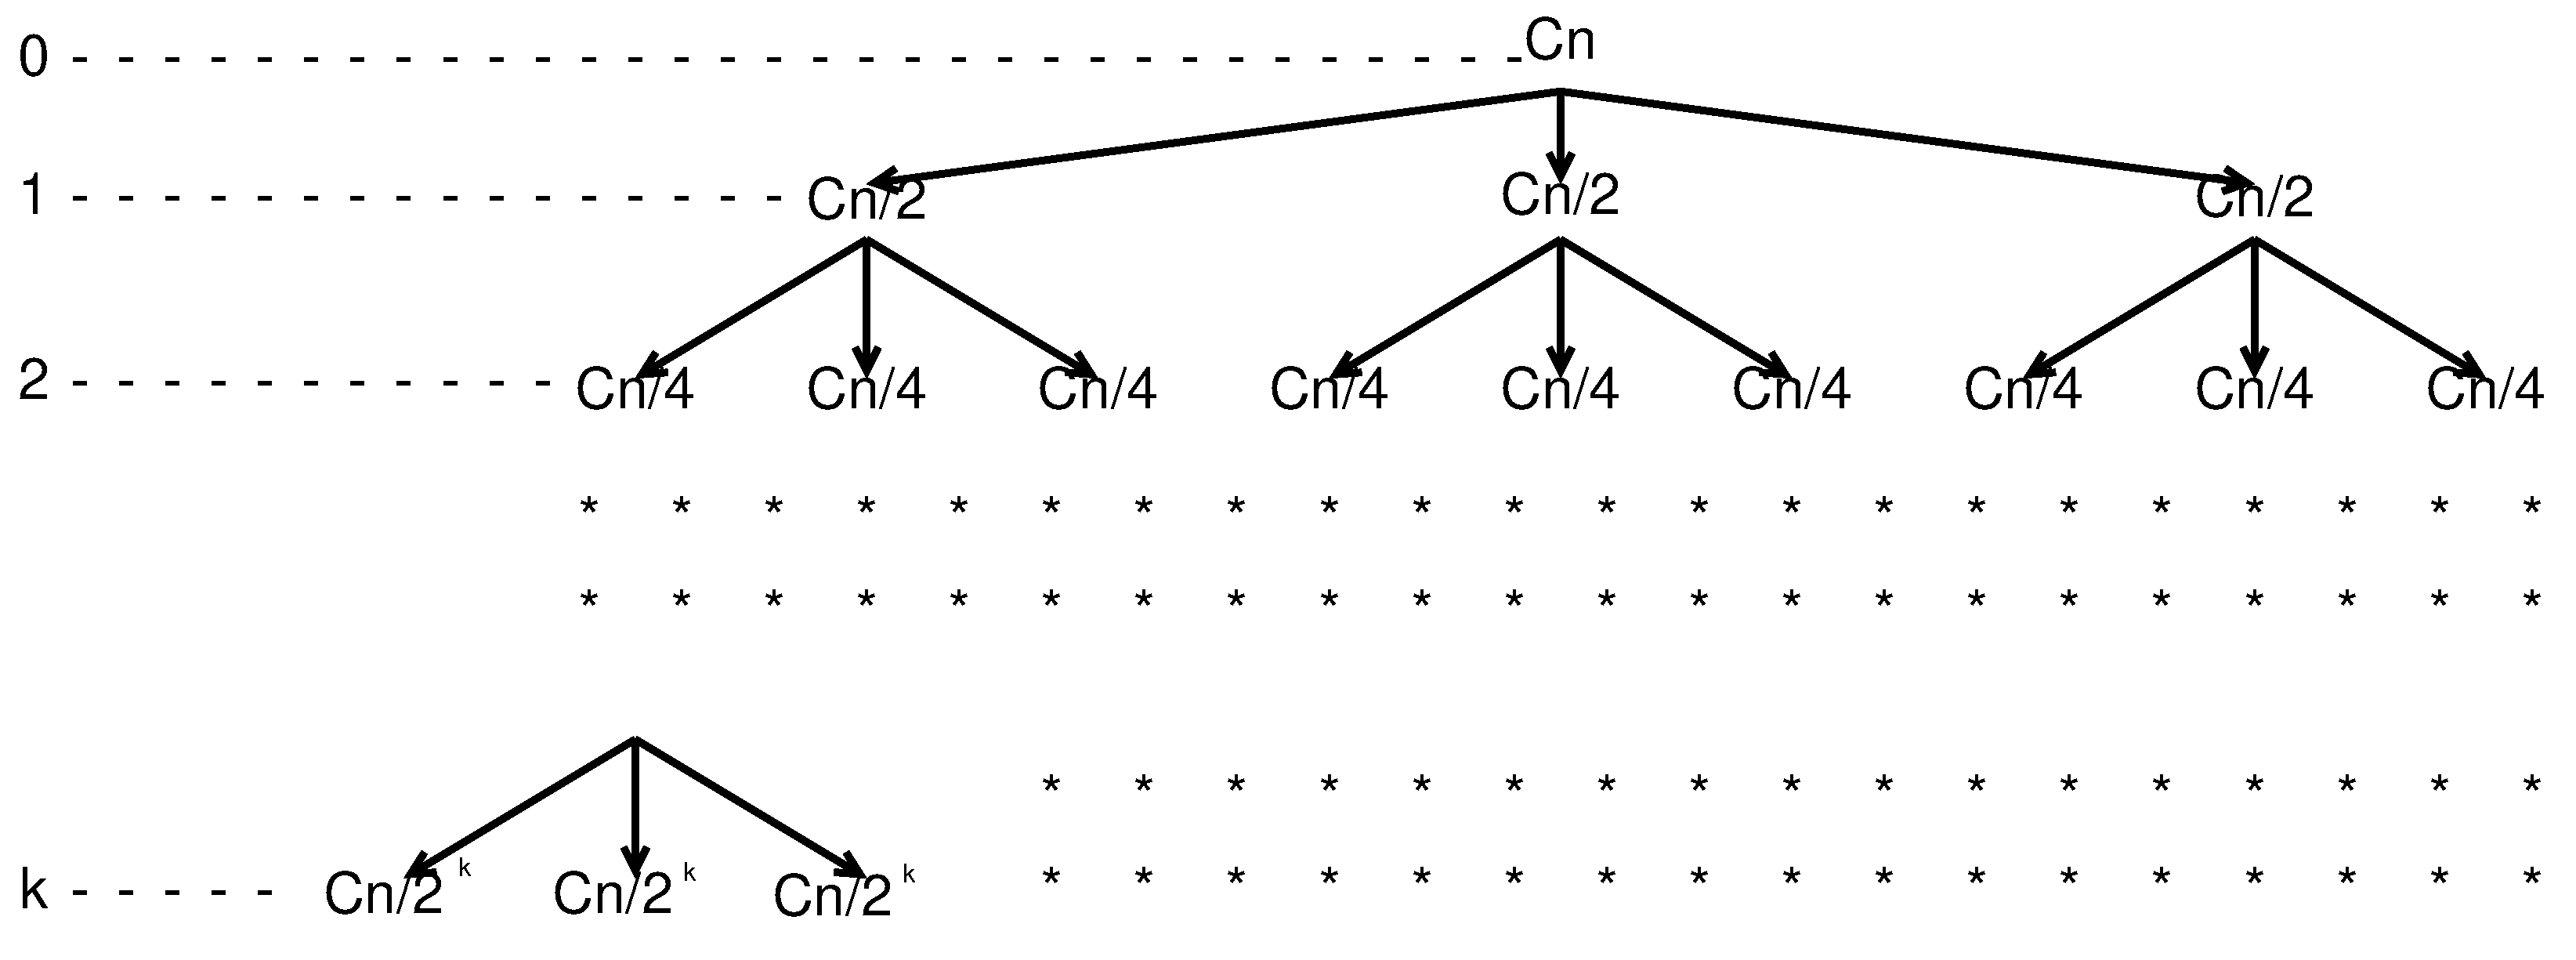
\includegraphics[width=\linewidth]{mul_tree}
	}
	\caption{Дерево рекурсии}
	\label{pic::mul_tree}
\end{figure}

Теперь по рисунку \ref{pic::mul_tree} можно сказать, что суммарное количество операций выполняемых на $i$-ом уровне:

\begin{equation}
	T_i^n = 3^iCn/2^i
\end{equation}

А по всем уровням:

\begin{equation}
	T(n) = \sum_{i=0}^{k=\log n} 3^iCn/2^i = Cn \sum_{i=0}^{k=\log n} \left(\frac{3}{2}\right)^i = \frac{Cn}{\frac{3}{2}-1}\left({\frac{3}{2}}^{k+1}-1\right) = \Theta (3^{\log n})
\end{equation}

Ну чтоже работа сделана, оценка улучшена, извлекаем из этого выводы, а вывод прост, что вообще говоря рекурсия вещь очень полезная, если конечно уметь ее аналаизировать. Реккурентные соотношения подобного класса (разделение исходной задачи на равные подзадачи) довольно часто встречаются в практике (большинство алгоритмов типа "разделяй и властвуй" описываются подобными соотношениями, а те что не описываются к ним очень близки), посему полезно иметь некий простой общий способ решения таких соотношений, получить такой спосбо не трудно, по схеме с деревом, давайте попробуем его вывести.

Пусть имеется алгоритм описываемый соотношением:
\begin{equation}
	T(n) = aT(n/b) + O(n^c) = aT(n/b) + Kn^c
\end{equation}

Построим для него аналогичное дерево.
\begin{figure}[h]
	\noindent\center{
		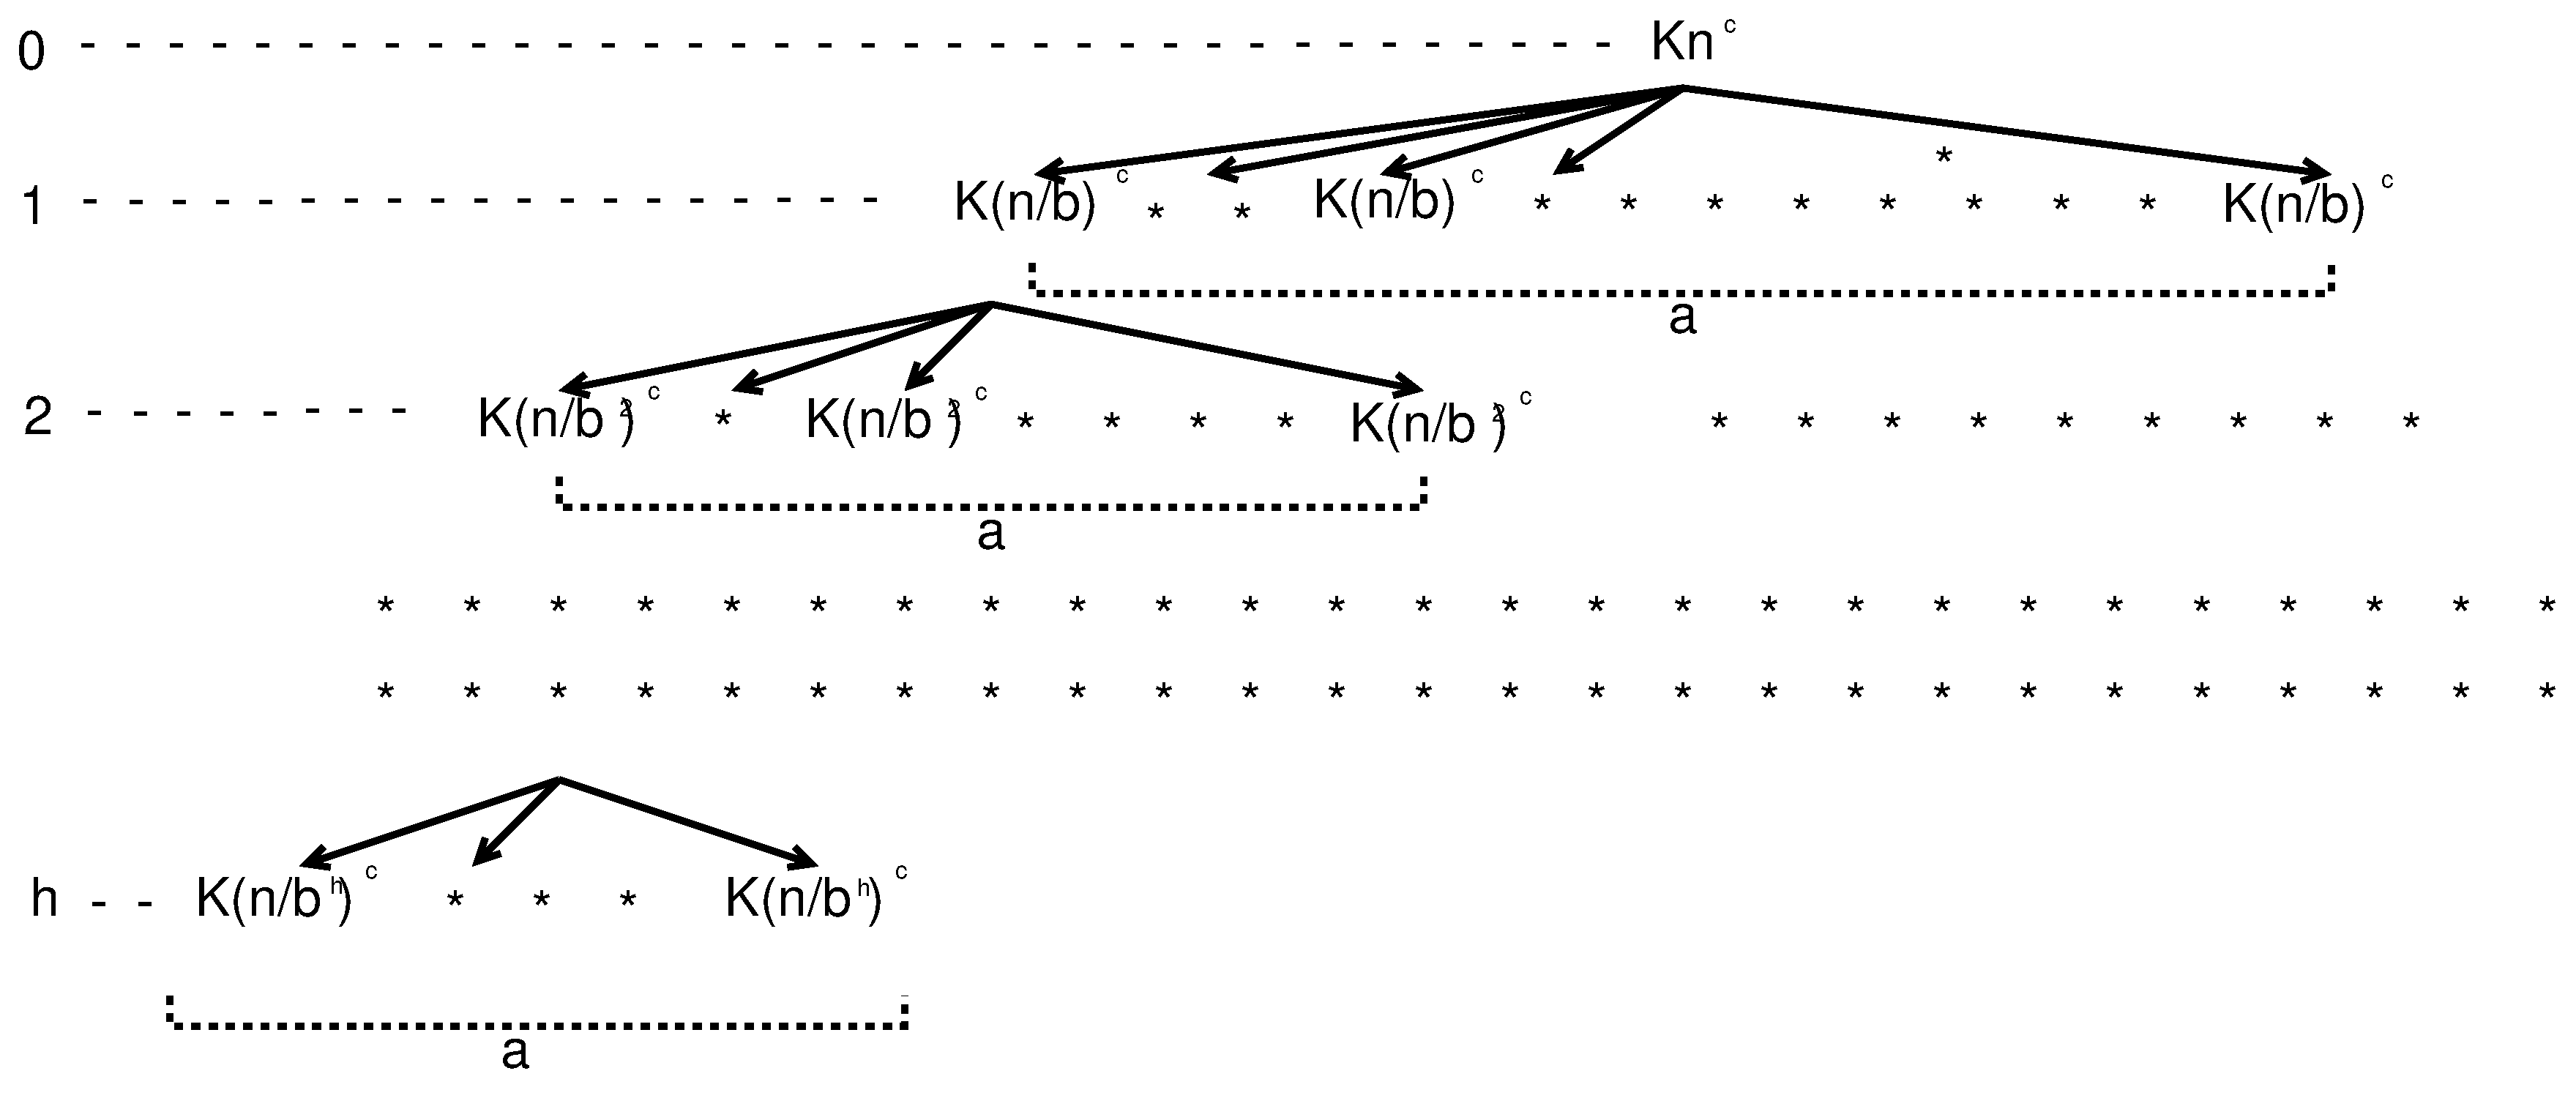
\includegraphics[width=\linewidth]{com_tree}
	}
	\caption{Дерево рекурсии}
	\label{pic::com_tree}
\end{figure}
На рисунке \ref{pic::com_tree} $h = \log_b n$ - высота дерева. Для $i$-ого уровня общая работа равна:

\begin{equation}
	T_i^n = {a^i}K\left({n}/{b^i}\right)^c
\end{equation}

просуммировав по всем уроням получаем:

\begin{equation}
	T(n) = \sum_{i=0}^{h=\log_b n} {a^i}K\left({n}/{b^i}\right)^c = K n^c \sum_{i=0}^{h=\log_b n} \left(\frac{a}{b^c}\right)^i
\end{equation}

Теперь рассмотрим отношение $\frac{a}{b^c}$, если:
\begin{enumerate}
\item $\log_b a > c$: $\frac{\log a}{c\log b} = \frac{\log_b a}{c} > 1$, откуда следует, что геометрическая прогрессия растет как последний член, $T(n) = K n^c \Theta \left(\left( \frac{a}{b^c} \right)^{\log_b n}\right) = \\ = K n^c \Theta \left(\frac{n^{\log_b a}}{n^c}\right) = O \left( n^{\log_b a} \right)$

\item $\log_b a = c$: по аналогии преобразуем геометрическую прогрессию в сумму констант и получаем $T(n) = K n^c O\Theta \left(\log_b n\right) = \Theta \left( n^c \log_b n \right)$

\item $\log_b a < c$: опять же по аналогии, подставляем прогрессию, увеличиваем верхний предел до бесконечности и считаем ее бесконечно убывающей, $T(n) = K n^c O \left(\sum_{i=0}^{\infty} \left(\frac{a}{b^c}\right)^i\right) = \Theta \left(\frac{K n^c}{1 - \frac{a}{b^c}}\right) = \Theta \left(n^c\right)$
\end{enumerate}

На сем, коротенькое ведение  рекурсивные выражения закончено
